\documentclass[a4paper,11pt]{article}
\usepackage{amsmath,amsthm,amsfonts,amssymb,amscd,amstext,vmargin,graphics,graphicx,tabularx,multicol} 
\usepackage[francais]{babel}
\usepackage[utf8]{inputenc}  
\usepackage[T1]{fontenc} 
\usepackage{pstricks-add,tikz,tkz-tab,variations}
\usepackage[autolanguage,np]{numprint} 

\setmarginsrb{1.5cm}{0.5cm}{1cm}{0.5cm}{0cm}{0cm}{0cm}{0cm} %Gauche, haut, droite, haut
\newcounter{numexo}
\newcommand{\exo}[1]{\stepcounter{numexo}\noindent{\bf Exercice~\thenumexo} : \marginpar{\hfill /#1}}
\reversemarginpar


\newcounter{enumtabi}
\newcounter{enumtaba}
\newcommand{\q}{\stepcounter{enumtabi} \theenumtabi)  }
\newcommand{\qa}{\stepcounter{enumtaba} (\alph{enumtaba}) }
\newcommand{\initq}{\setcounter{enumtabi}{0}}
\newcommand{\initqa}{\setcounter{enumtaba}{0}}

\newcommand{\be}{\begin{enumerate}}
\newcommand{\ee}{\end{enumerate}}
\newcommand{\bi}{\begin{itemize}}
\newcommand{\ei}{\end{itemize}}
\newcommand{\bp}{\begin{pspicture*}}
\newcommand{\ep}{\end{pspicture*}}
\newcommand{\bt}{\begin{tabular}}
\newcommand{\et}{\end{tabular}}
\renewcommand{\tabularxcolumn}[1]{>{\centering}m{#1}} %(colonne m{} centrée, au lieu de p par défault) 
\newcommand{\tnl}{\tabularnewline}

\newcommand{\bmul}[1]{\begin{multicols}{#1}}
\newcommand{\emul}{\end{multicols}}

\newcommand{\trait}{\noindent \rule{\linewidth}{0.2mm}}
\newcommand{\hs}[1]{\hspace{#1}}
\newcommand{\vs}[1]{\vspace{#1}}

\newcommand{\N}{\mathbb{N}}
\newcommand{\Z}{\mathbb{Z}}
\newcommand{\R}{\mathbb{R}}
\newcommand{\C}{\mathbb{C}}
\newcommand{\Dcal}{\mathcal{D}}
\newcommand{\Ccal}{\mathcal{C}}
\newcommand{\mc}{\mathcal}

\newcommand{\vect}[1]{\overrightarrow{#1}}
\newcommand{\ds}{\displaystyle}
\newcommand{\eq}{\quad \Leftrightarrow \quad}
\newcommand{\vecti}{\vec{\imath}}
\newcommand{\vectj}{\vec{\jmath}}
\newcommand{\Oij}{(O;\vec{\imath}, \vec{\jmath})}
\newcommand{\OIJ}{(O;I,J)}


\newcommand{\reponse}[1][1]{%
\multido{}{#1}{\makebox[\linewidth]{\rule[0pt]{0pt}{20pt}\dotfill}
}}

\newcommand{\titre}[5] 
% #1: titre #2: haut gauche #3: bas gauche #4: haut droite #5: bas droite
{
\noindent #2 \hfill #4 \\
#3 \hfill #5

\vspace{-1.6cm}

\begin{center}\rule{6cm}{0.5mm}\end{center}
\vspace{0.2cm}
\begin{center}{\large{\textbf{#1}}}\end{center}
\begin{center}\rule{6cm}{0.5mm}\end{center}
}



\begin{document}
\pagestyle{empty}
\titre{Contrôle 1}{Nom :}{Prénom :}{Classe}{Date}




\exo{3} \textit{(Les fractions)}\\
 Calculer les expressions suivantes et donner la réponse \textbf{sous forme d'une fraction irréductible.
}
\bmul{2}



$K = \dfrac{3}{6} - \dfrac{5}{30}+\dfrac{1}{15}$\\






\columnbreak


$S = \left(\dfrac{2}{7}+\dfrac{7}{2}\right)-\left(\dfrac{5}{8}-1\right)$ \\
\emul

\vspace*{0.25cm}




\exo{2} \textit{(Proportionnalité)}


Un avionneur donne la consommation moyenne de l'un de ses avions moyen courrier grâce au graphique ci-dessous.
\begin{center}


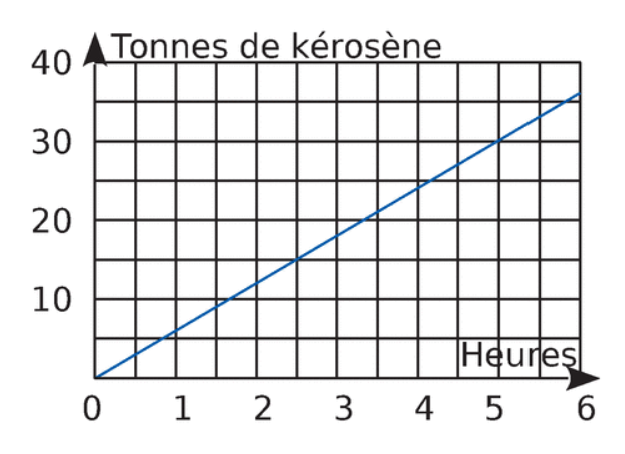
\includegraphics[scale=0.7]{avionneur.eps} 
\end{center}

\qa La quantité de kérosène et le temps passé dans les airs  sont-ils proportionnels  ? \textit{Expliquer}.\\

\qa	A l'aide du graphique, donner le plus précisément possible la quantité de kérosène nécessaire pour faire voler un avion pendant 2 heures 30.\\

\vspace*{0.75cm}

\exo{4} \textit{(Les transformations)}
\bmul{2}
\initq
\q On considère l'hexagone ABCDEF de centre O représenté ci-contre.\\

\initqa \qa Quelle est l'image du quadrilatère FABO par la symétrie de centre O?\\

\qa Quelle est l'image du segment [BO] par la symétrie d'axe (CF)?\\

\qa On considère la rotation de centre O qui transforme le triangle OAB en le triangle OCD.\\
Quelle est l'image du triangle BOC par cette rotation ?\\


\columnbreak

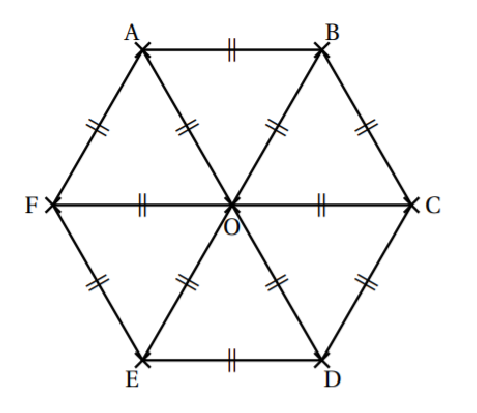
\includegraphics[scale=0.8]{hexagone1.eps} 

\emul


\bmul{2}
\q La figure ci-contre représente un pavage dont le motif
de base a la même forme que l'hexagone ci-dessus. On
a numéroté certains de ces hexagones.\\
$\rightarrow$ \textbf{Quelle est l'image de l'hexagone 9 par la translation qui transforme l'hexagone 2 en l'hexagone
12 ?}\\

\columnbreak

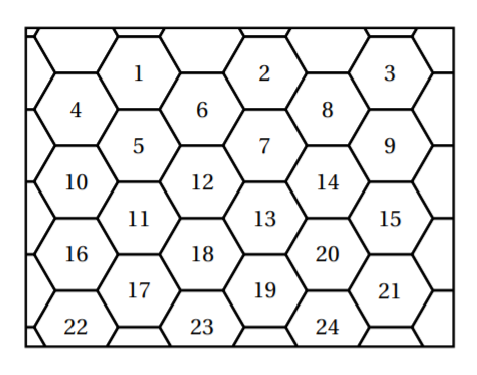
\includegraphics[scale=0.7]{nidabeille.eps} 

\vspace*{0.75cm}


\emul

\vspace*{0.5cm}


\exo{5} Un professeur de SVT demande aux élèves d'une classe de sixième de faire germer des graines de blé chez eux.\\

Le professeur donne un protocole expérimental à suivre.
\bi
\item Mettre en culture sur du coton dans une boîte placée dans une pièce éclairée, de température entre \\
20  C et 25 C.
\item Arroser une fois par jour.
\item Il est possible de couvrir les graines avec un film transparent pour éviter l'évaporation de l'eau.\\
\ei

Le tableau ci-dessous donne les tailles des plantules (petites plantes) des élèves à 10 jours après la mise en germination.\\


\renewcommand{\arraystretch}{1.8}

\begin{tabular}{|c|c|c|c|c|c|c|c|c|c|c|c|}
\hline 
Taille (en cm) & 0 & 8 & 12 & 14 & 16 & 17 & 18 & 19 & 20 & 21 & 22 \\ 
\hline 
Effectifs & 1 & 2 & 2 & 4 & 2 & 2 & 3 & 3 & 4 & 4 & 2 \\ 
\hline 
\end{tabular} 

\vspace*{0.4cm}

\textbf{QUESTIONS :}\\
\initq \q Quel est effectif total de cette série ?\\
\q Quel pourcentage des élèves de la classe a obtenu une plantule qui mesure au plus 17 cm ? \textit{(17 inclus)}\\
\q On considère qu'un élève a bien respecté le protocole si la taille de la plantule à 10 jours est supérieure ou égale à 14 cm.\\
Quel pourcentage des élèves de la classe a bien respecté le protocole ?\\
\q Quelle est la taille moyenne des plantules de cette classe de $6^{eme}$ ?\\


\exo{6}
L'histogramme ci-dessous donne la répartition des habitants d'une commune en fonction de leur âge. 

\begin{center}
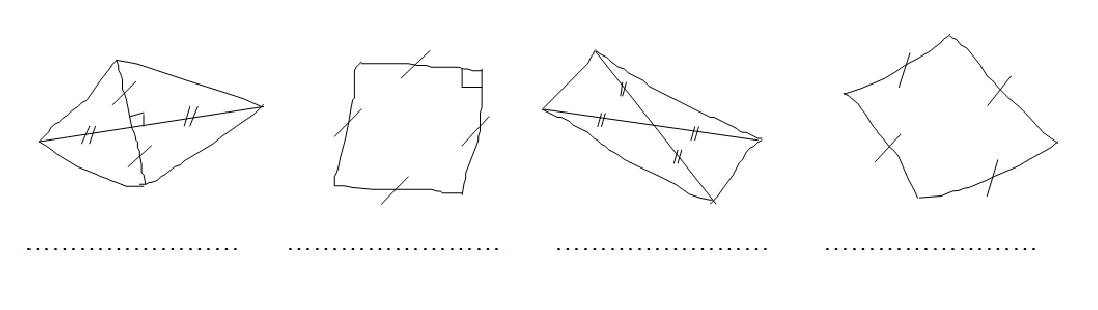
\includegraphics[scale=0.7]{interro1.eps} 
\end{center}

Voici un tableau qui représente la situation :\\

\renewcommand{\arraystretch}{2}

\begin{tabular}{|c|c|c|c|c|c|}
\hline 
Ages des habitants (en années) & \hspace*{0.3cm} [0;20[ \hspace*{0.3cm}& \hspace*{0.3cm} [20;40[ \hspace*{0.3cm} & \hspace*{0.3cm} [40;60[ \hspace*{0.3cm} & \hspace*{0.3cm} [60;80[ \hspace*{0.3cm} &\hspace*{0.3cm} [80;100[ \hspace*{0.3cm}\\ 
\hline 
Effectifs &  &  &  &  &  \\ 
\hline 
Fréquences (en pourcentage) &  &  &  &  &  \\ 
\hline 
\end{tabular} 

\vspace*{0.4cm}

\textbf{QUESTIONS :}\\
\initq \q Compléter le tableau ci-dessus. (\textit{sans justification})\\
\q Quel est l'effectif total dans cette série statistique ? \\
\q Quelle est la fréquence en pourcentage du nombre d'habitants ayant moins de 40 ans \textit{(40 ans exlus)} ? \\
\q Quelle est la moyenne d'âges des habitants de cette commune ? \\

\end{document}
